\section{Consigna}

Calcule el circuito adaptador de impedancias mostrado en la Fig. . Considerar que la impedancia de entrada es de $50 \: [\Omega]$ y la impedancia de salida es de $600 \: [\Omega]$. Calcule $Q_{t}$, $L_{1}$ y $C_{1}$ para una frecuencia de trabajo de $10 \: [MHz]$.

\begin{figure}
  \centering
  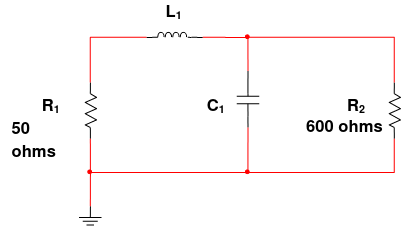
\includegraphics[width=0.5\textwidth]{../images/eje1_circuito.png}
  \caption{Adaptador 1}
  \label{fig:eje1_circuito}

\end{figure}
